
%% bare_jrnl.tex
%% V1.3
%% 2007/01/11
%% by Michael Shell
%% see http://www.michaelshell.org/
%% for current contact information.
%%
%% This is a skeleton file demonstrating the use of IEEEtran.cls
%% (requires IEEEtran.cls version 1.7 or later) with an IEEE journal paper.
%%
%% Support sites:
%% http://www.michaelshell.org/tex/ieeetran/
%% http://www.ctan.org/tex-archive/macros/latex/contrib/IEEEtran/
%% and
%% http://www.ieee.org/



% *** Authors should verify (and, if needed, correct) their LaTeX system  ***
% *** with the testflow diagnostic prior to trusting their LaTeX platform ***
% *** with production work. IEEE's font choices can trigger bugs that do  ***
% *** not appear when using other class files.                            ***
% The testflow support page is at:
% http://www.michaelshell.org/tex/testflow/


%%*************************************************************************
%% Legal Notice:
%% This code is offered as-is without any warranty either expressed or
%% implied; without even the implied warranty of MERCHANTABILITY or
%% FITNESS FOR A PARTICULAR PURPOSE!
%% User assumes all risk.
%% In no event shall IEEE or any contributor to this code be liable for
%% any damages or losses, including, but not limited to, incidental,
%% consequential, or any other damages, resulting from the use or misuse
%% of any information contained here.
%%
%% All comments are the opinions of their respective authors and are not
%% necessarily endorsed by the IEEE.
%%
%% This work is distributed under the LaTeX Project Public License (LPPL)
%% ( http://www.latex-project.org/ ) version 1.3, and may be freely used,
%% distributed and modified. A copy of the LPPL, version 1.3, is included
%% in the base LaTeX documentation of all distributions of LaTeX released
%% 2003/12/01 or later.
%% Retain all contribution notices and credits.
%% ** Modified files should be clearly indicated as such, including  **
%% ** renaming them and changing author support contact information. **
%%
%% File list of work: IEEEtran.cls, IEEEtran_HOWTO.pdf, bare_adv.tex,
%%                    bare_conf.tex, bare_jrnl.tex, bare_jrnl_compsoc.tex
%%*************************************************************************

% Note that the a4paper option is mainly intended so that authors in
% countries using A4 can easily print to A4 and see how their papers will
% look in print - the typesetting of the document will not typically be
% affected with changes in paper size (but the bottom and side margins will).
% Use the testflow package mentioned above to verify correct handling of
% both paper sizes by the user's LaTeX system.
%
% Also note that the "draftcls" or "draftclsnofoot", not "draft", option
% should be used if it is desired that the figures are to be displayed in
% draft mode.
%
\documentclass[journal]{IEEEtran}
\usepackage{blindtext}
\usepackage{graphicx}

% Some very useful LaTeX packages include:
% (uncomment the ones you want to load)


% *** MISC UTILITY PACKAGES ***
%
%\usepackage{ifpdf}
% Heiko Oberdiek's ifpdf.sty is very useful if you need conditional
% compilation based on whether the output is pdf or dvi.
% usage:
% \ifpdf
%   % pdf code
% \else
%   % dvi code
% \fi
% The latest version of ifpdf.sty can be obtained from:
% http://www.ctan.org/tex-archive/macros/latex/contrib/oberdiek/
% Also, note that IEEEtran.cls V1.7 and later provides a builtin
% \ifCLASSINFOpdf conditional that works the same way.
% When switching from latex to pdflatex and vice-versa, the compiler may
% have to be run twice to clear warning/error messages.






% *** CITATION PACKAGES ***
%
%\usepackage{cite}
% cite.sty was written by Donald Arseneau
% V1.6 and later of IEEEtran pre-defines the format of the cite.sty package
% \cite{} output to follow that of IEEE. Loading the cite package will
% result in citation numbers being automatically sorted and properly
% "compressed/ranged". e.g., [1], [9], [2], [7], [5], [6] without using
% cite.sty will become [1], [2], [5]--[7], [9] using cite.sty. cite.sty's
% \cite will automatically add leading space, if needed. Use cite.sty's
% noadjust option (cite.sty V3.8 and later) if you want to turn this off.
% cite.sty is already installed on most LaTeX systems. Be sure and use
% version 4.0 (2003-05-27) and later if using hyperref.sty. cite.sty does
% not currently provide for hyperlinked citations.
% The latest version can be obtained at:
% http://www.ctan.org/tex-archive/macros/latex/contrib/cite/
% The documentation is contained in the cite.sty file itself.






% *** GRAPHICS RELATED PACKAGES ***
%
\ifCLASSINFOpdf
  % \usepackage[pdftex]{graphicx}
  % declare the path(s) where your graphic files are
  % \graphicspath{{../pdf/}{../jpeg/}}
  % and their extensions so you won't have to specify these with
  % every instance of \includegraphics
  % \DeclareGraphicsExtensions{.pdf,.jpeg,.png}
\else
  % or other class option (dvipsone, dvipdf, if not using dvips). graphicx
  % will default to the driver specified in the system graphics.cfg if no
  % driver is specified.
  % \usepackage[dvips]{graphicx}
  % declare the path(s) where your graphic files are
  % \graphicspath{{../eps/}}
  % and their extensions so you won't have to specify these with
  % every instance of \includegraphics
  % \DeclareGraphicsExtensions{.eps}
\fi
% graphicx was written by David Carlisle and Sebastian Rahtz. It is
% required if you want graphics, photos, etc. graphicx.sty is already
% installed on most LaTeX systems. The latest version and documentation can
% be obtained at:
% http://www.ctan.org/tex-archive/macros/latex/required/graphics/
% Another good source of documentation is "Using Imported Graphics in
% LaTeX2e" by Keith Reckdahl which can be found as epslatex.ps or
% epslatex.pdf at: http://www.ctan.org/tex-archive/info/
%
% latex, and pdflatex in dvi mode, support graphics in encapsulated
% postscript (.eps) format. pdflatex in pdf mode supports graphics
% in .pdf, .jpeg, .png and .mps (metapost) formats. Users should ensure
% that all non-photo figures use a vector format (.eps, .pdf, .mps) and
% not a bitmapped formats (.jpeg, .png). IEEE frowns on bitmapped formats
% which can result in "jaggedy"/blurry rendering of lines and letters as
% well as large increases in file sizes.
%
% You can find documentation about the pdfTeX application at:
% http://www.tug.org/applications/pdftex





% *** MATH PACKAGES ***
%
%\usepackage[cmex10]{amsmath}
% A popular package from the American Mathematical Society that provides
% many useful and powerful commands for dealing with mathematics. If using
% it, be sure to load this package with the cmex10 option to ensure that
% only type 1 fonts will utilized at all point sizes. Without this option,
% it is possible that some math symbols, particularly those within
% footnotes, will be rendered in bitmap form which will result in a
% document that can not be IEEE Xplore compliant!
%
% Also, note that the amsmath package sets \interdisplaylinepenalty to 10000
% thus preventing page breaks from occurring within multiline equations. Use:
%\interdisplaylinepenalty=2500
% after loading amsmath to restore such page breaks as IEEEtran.cls normally
% does. amsmath.sty is already installed on most LaTeX systems. The latest
% version and documentation can be obtained at:
% http://www.ctan.org/tex-archive/macros/latex/required/amslatex/math/





% *** SPECIALIZED LIST PACKAGES ***
%
%\usepackage{algorithmic}
% algorithmic.sty was written by Peter Williams and Rogerio Brito.
% This package provides an algorithmic environment fo describing algorithms.
% You can use the algorithmic environment in-text or within a figure
% environment to provide for a floating algorithm. Do NOT use the algorithm
% floating environment provided by algorithm.sty (by the same authors) or
% algorithm2e.sty (by Christophe Fiorio) as IEEE does not use dedicated
% algorithm float types and packages that provide these will not provide
% correct IEEE style captions. The latest version and documentation of
% algorithmic.sty can be obtained at:
% http://www.ctan.org/tex-archive/macros/latex/contrib/algorithms/
% There is also a support site at:
% http://algorithms.berlios.de/index.html
% Also of interest may be the (relatively newer and more customizable)
% algorithmicx.sty package by Szasz Janos:
% http://www.ctan.org/tex-archive/macros/latex/contrib/algorithmicx/




% *** ALIGNMENT PACKAGES ***
%
%\usepackage{array}
% Frank Mittelbach's and David Carlisle's array.sty patches and improves
% the standard LaTeX2e array and tabular environments to provide better
% appearance and additional user controls. As the default LaTeX2e table
% generation code is lacking to the point of almost being broken with
% respect to the quality of the end results, all users are strongly
% advised to use an enhanced (at the very least that provided by array.sty)
% set of table tools. array.sty is already installed on most systems. The
% latest version and documentation can be obtained at:
% http://www.ctan.org/tex-archive/macros/latex/required/tools/


%\usepackage{mdwmath}
%\usepackage{mdwtab}
% Also highly recommended is Mark Wooding's extremely powerful MDW tools,
% especially mdwmath.sty and mdwtab.sty which are used to format equations
% and tables, respectively. The MDWtools set is already installed on most
% LaTeX systems. The lastest version and documentation is available at:
% http://www.ctan.org/tex-archive/macros/latex/contrib/mdwtools/


% IEEEtran contains the IEEEeqnarray family of commands that can be used to
% generate multiline equations as well as matrices, tables, etc., of high
% quality.


%\usepackage{eqparbox}
% Also of notable interest is Scott Pakin's eqparbox package for creating
% (automatically sized) equal width boxes - aka "natural width parboxes".
% Available at:
% http://www.ctan.org/tex-archive/macros/latex/contrib/eqparbox/





% *** SUBFIGURE PACKAGES ***
%\usepackage[tight,footnotesize]{subfigure}
% subfigure.sty was written by Steven Douglas Cochran. This package makes it
% easy to put subfigures in your figures. e.g., "Figure 1a and 1b". For IEEE
% work, it is a good idea to load it with the tight package option to reduce
% the amount of white space around the subfigures. subfigure.sty is already
% installed on most LaTeX systems. The latest version and documentation can
% be obtained at:
% http://www.ctan.org/tex-archive/obsolete/macros/latex/contrib/subfigure/
% subfigure.sty has been superceeded by subfig.sty.



%\usepackage[caption=false]{caption}
%\usepackage[font=footnotesize]{subfig}
% subfig.sty, also written by Steven Douglas Cochran, is the modern
% replacement for subfigure.sty. However, subfig.sty requires and
% automatically loads Axel Sommerfeldt's caption.sty which will override
% IEEEtran.cls handling of captions and this will result in nonIEEE style
% figure/table captions. To prevent this problem, be sure and preload
% caption.sty with its "caption=false" package option. This is will preserve
% IEEEtran.cls handing of captions. Version 1.3 (2005/06/28) and later
% (recommended due to many improvements over 1.2) of subfig.sty supports
% the caption=false option directly:
%\usepackage[caption=false,font=footnotesize]{subfig}
%
% The latest version and documentation can be obtained at:
% http://www.ctan.org/tex-archive/macros/latex/contrib/subfig/
% The latest version and documentation of caption.sty can be obtained at:
% http://www.ctan.org/tex-archive/macros/latex/contrib/caption/




% *** FLOAT PACKAGES ***
%
%\usepackage{fixltx2e}
% fixltx2e, the successor to the earlier fix2col.sty, was written by
% Frank Mittelbach and David Carlisle. This package corrects a few problems
% in the LaTeX2e kernel, the most notable of which is that in current
% LaTeX2e releases, the ordering of single and double column floats is not
% guaranteed to be preserved. Thus, an unpatched LaTeX2e can allow a
% single column figure to be placed prior to an earlier double column
% figure. The latest version and documentation can be found at:
% http://www.ctan.org/tex-archive/macros/latex/base/



%\usepackage{stfloats}
% stfloats.sty was written by Sigitas Tolusis. This package gives LaTeX2e
% the ability to do double column floats at the bottom of the page as well
% as the top. (e.g., "\begin{figure*}[!b]" is not normally possible in
% LaTeX2e). It also provides a command:
%\fnbelowfloat
% to enable the placement of footnotes below bottom floats (the standard
% LaTeX2e kernel puts them above bottom floats). This is an invasive package
% which rewrites many portions of the LaTeX2e float routines. It may not work
% with other packages that modify the LaTeX2e float routines. The latest
% version and documentation can be obtained at:
% http://www.ctan.org/tex-archive/macros/latex/contrib/sttools/
% Documentation is contained in the stfloats.sty comments as well as in the
% presfull.pdf file. Do not use the stfloats baselinefloat ability as IEEE
% does not allow \baselineskip to stretch. Authors submitting work to the
% IEEE should note that IEEE rarely uses double column equations and
% that authors should try to avoid such use. Do not be tempted to use the
% cuted.sty or midfloat.sty packages (also by Sigitas Tolusis) as IEEE does
% not format its papers in such ways.


%\ifCLASSOPTIONcaptionsoff
%  \usepackage[nomarkers]{endfloat}
% \let\MYoriglatexcaption\caption
% \renewcommand{\caption}[2][\relax]{\MYoriglatexcaption[#2]{#2}}
%\fi
% endfloat.sty was written by James Darrell McCauley and Jeff Goldberg.
% This package may be useful when used in conjunction with IEEEtran.cls'
% captionsoff option. Some IEEE journals/societies require that submissions
% have lists of figures/tables at the end of the paper and that
% figures/tables without any captions are placed on a page by themselves at
% the end of the document. If needed, the draftcls IEEEtran class option or
% \CLASSINPUTbaselinestretch interface can be used to increase the line
% spacing as well. Be sure and use the nomarkers option of endfloat to
% prevent endfloat from "marking" where the figures would have been placed
% in the text. The two hack lines of code above are a slight modification of
% that suggested by in the endfloat docs (section 8.3.1) to ensure that
% the full captions always appear in the list of figures/tables - even if
% the user used the short optional argument of \caption[]{}.
% IEEE papers do not typically make use of \caption[]'s optional argument,
% so this should not be an issue. A similar trick can be used to disable
% captions of packages such as subfig.sty that lack options to turn off
% the subcaptions:
% For subfig.sty:
% \let\MYorigsubfloat\subfloat
% \renewcommand{\subfloat}[2][\relax]{\MYorigsubfloat[]{#2}}
% For subfigure.sty:
% \let\MYorigsubfigure\subfigure
% \renewcommand{\subfigure}[2][\relax]{\MYorigsubfigure[]{#2}}
% However, the above trick will not work if both optional arguments of
% the \subfloat/subfig command are used. Furthermore, there needs to be a
% description of each subfigure *somewhere* and endfloat does not add
% subfigure captions to its list of figures. Thus, the best approach is to
% avoid the use of subfigure captions (many IEEE journals avoid them anyway)
% and instead reference/explain all the subfigures within the main caption.
% The latest version of endfloat.sty and its documentation can obtained at:
% http://www.ctan.org/tex-archive/macros/latex/contrib/endfloat/
%
% The IEEEtran \ifCLASSOPTIONcaptionsoff conditional can also be used
% later in the document, say, to conditionally put the References on a
% page by themselves.





% *** PDF, URL AND HYPERLINK PACKAGES ***
%
%\usepackage{url}
% url.sty was written by Donald Arseneau. It provides better support for
% handling and breaking URLs. url.sty is already installed on most LaTeX
% systems. The latest version can be obtained at:
% http://www.ctan.org/tex-archive/macros/latex/contrib/misc/
% Read the url.sty source comments for usage information. Basically,
% \url{my_url_here}.





% *** Do not adjust lengths that control margins, column widths, etc. ***
% *** Do not use packages that alter fonts (such as pslatex).         ***
% There should be no need to do such things with IEEEtran.cls V1.6 and later.
% (Unless specifically asked to do so by the journal or conference you plan
% to submit to, of course. )


% correct bad hyphenation here
\hyphenation{}


\begin{document}
%
% paper title
% can use linebreaks \\ within to get better formatting as desired
\title{CS262 Pset2 Lab Notebook \\ \large https://github.com/ankitvgupta/cs262}
%
%
% author names and IEEE memberships
% note positions of commas and nonbreaking spaces ( ~ ) LaTeX will not break
% a structure at a ~ so this keeps an author's name from being broken across
% two lines.
% use \thanks{} to gain access to the first footnote area
% a separate \thanks must be used for each paragraph as LaTeX2e's \thanks
% was not built to handle multiple paragraphs
%

\author{Ankit Gupta, Jared Pochtar}


% make the title area
\maketitle

\section{High level Design - Python}
\begin{enumerate}
  \item Use Python multiprocessing to split into several processes
  \item Use multiprocessing.Queue to communicate between processes
  \item In each process
  \begin{enumerate}
    \item At the beginning, determine a sleep time.
    \item Until killed:
    \begin{enumerate}
      \item Sleep for process’s sleep time
      \item Wake, pull everything from interprocess queue into local queue
      \item Check if anything in local queue, if so, do work as specificed in the spec
    \end{enumerate}
  \end{enumerate}
  \item We make sure to always sleep for just enough time. In other words, if the sleep time is .5 seconds (meaning the clock speed is 2/second), and the work takes .2 seconds, then the sleep will only take .3 seconds to make up for this.
\end{enumerate}

Then, we took the data, and used Excel to quickly manipulate it, and visualize the increases in the logical clocks.

We actually decided to write the Python code in two ways. Let the time between ticks be k. In the method, described above, we only wake up every k seconds, and then do all of our work there, including pulling from the queue. This works, because we account for the time spent pulling from the queue later, but reducing the length of later sleeps so that the ticks are still every k seconds.

In the second method, we follow a similar approach, but instead we block until an item is inserted into a queue by another process, with a timeout of k. If an item into the interprocess queue in j < k seconds, we move it to a process-local buffer, and then block for k-j seconds. We repeat this process until a total of k seconds have passed from the last tick. This allows us to quickly move items from the interprocess queue into the local queue, while performing the logical clock work at the start of every kth second.

You can verify that our code does indeed do operations every k seconds by looking at the global time stamps, and noticing that it does maintain that pattern.

Next, in order to make running tests easy, we exposed several command line arguments. One was called the probability of a machine to take an internal action.  Another was controlled the maximum number of ticks per second of the clock of a process. The clock speed of a process in ticks per second is sampled uniformly between 1 and the max speed. Lastly, we exposed a parameter that determines how long the processes will run. We generally set this to be 60 seconds, as suggested in the specification.

\subsection{Problems along the way}
Originally, we just printing log results directly to stdout from each of the processes, and we would just pipe stdout into a file to keep a log. However, this did not work well with multiple processes as lines were occasionally overwritten or partially overwritten. Thus, we instead created a separate log for each of the processes, and then concatenate them afterwards. Lastly, we sorted the items in the log by the global system time, and generated two graphs. The first graph shows the size of the queue in each process at time point. The second graph shows the value of the logical clock for each process at each time point. This allowed us to see how the values of the logical clock and size of the queue change over time, and this setup proved crucial later in our analysis. The x axis of these graphs is always the global system clock time, and the y axis is either the queue length or the logical clock value, depending on the graph.

\section{Experimental Observations}

\subsection{Experiments 1}

In the first set of experiments, we used the default set of parameters.  This means that the number of ticks per second were between 1 and 6, and the values 4-10 were used for internal events.

All of the graphs for these three had the same overall look, and they appear as in the graph you can see at \ref{fig:ex1}

\begin{figure}[!ht]
  \label{fig:ex1}
  \centering
  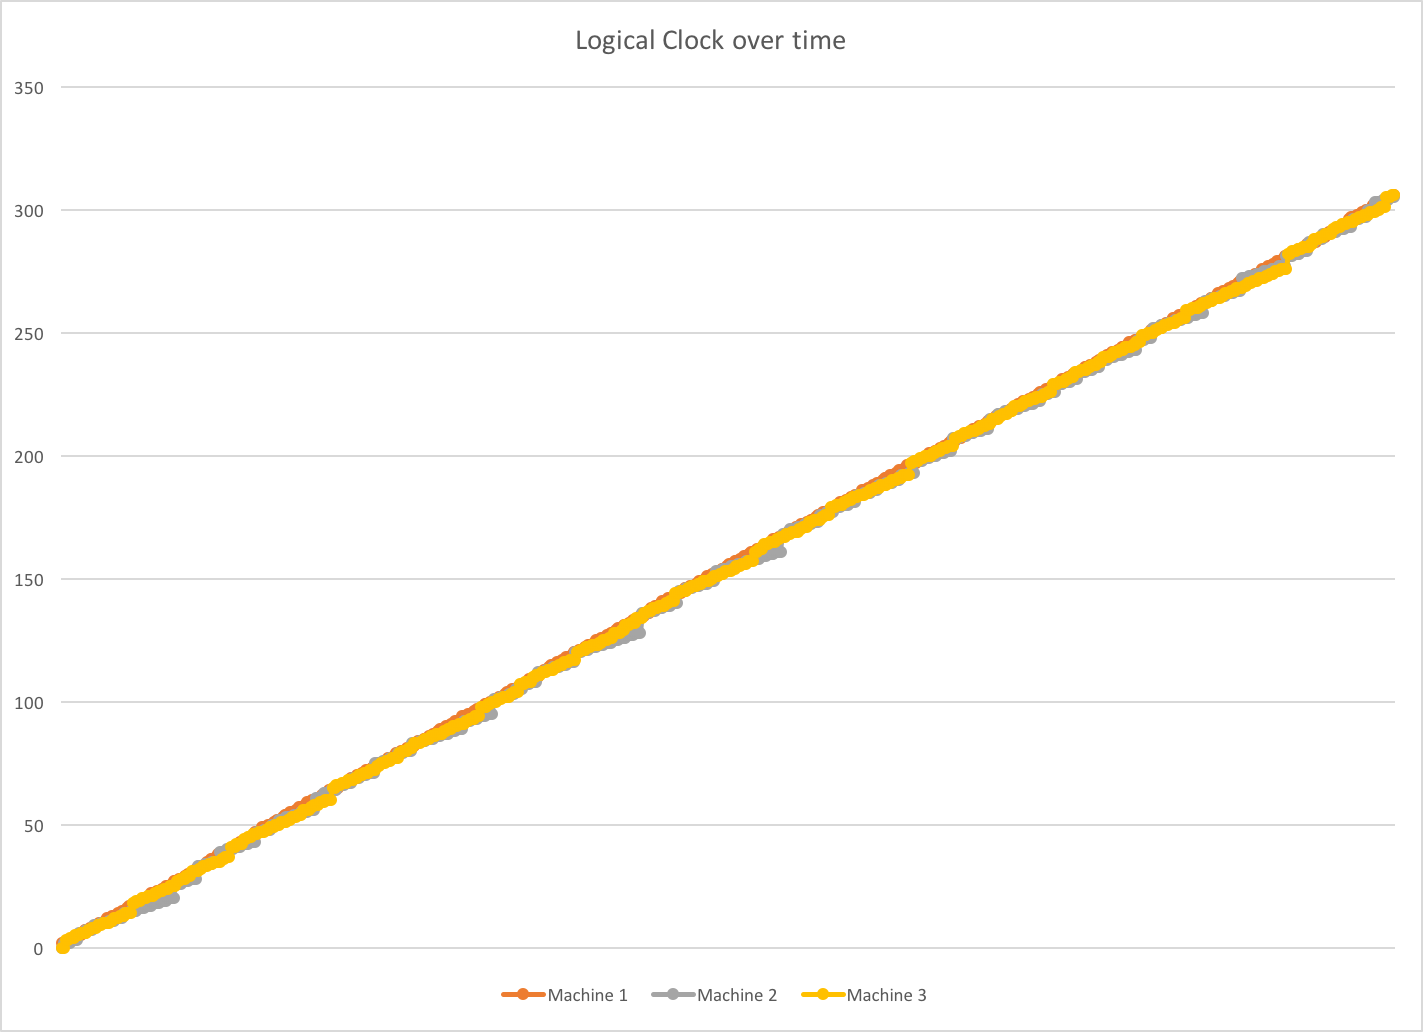
\includegraphics[width=0.5\textwidth]{{{pictures/1457670968.98_lc}}}
    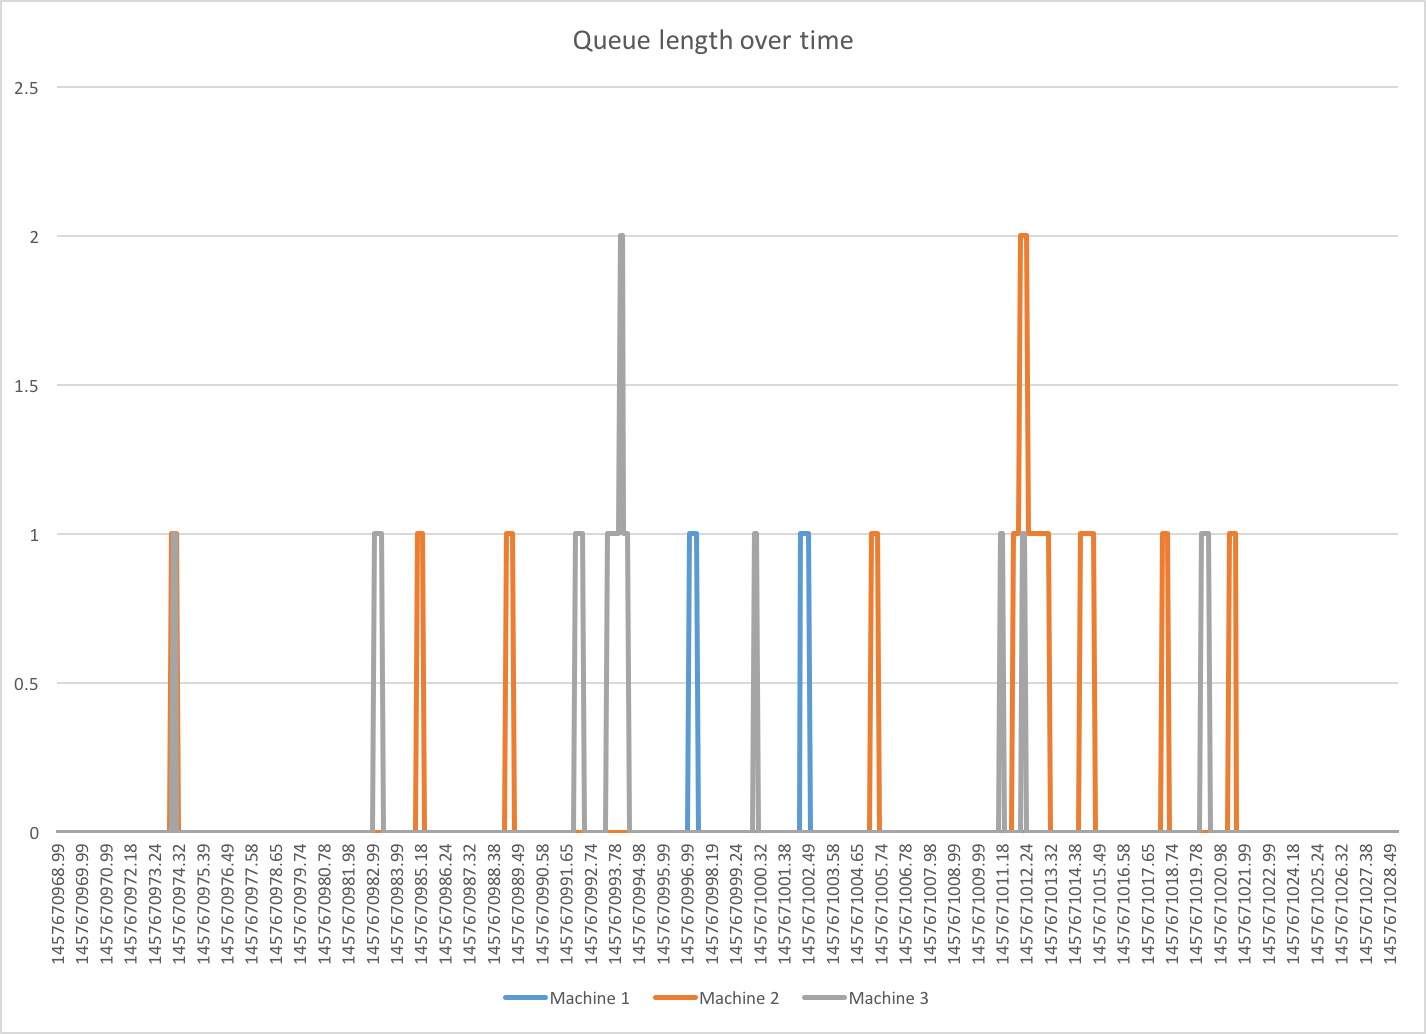
\includegraphics[width=0.5\textwidth]{{{pictures/1457670968.98_queue}}}
\end{figure}



In general, we can see that all three of the processes are generally able to keep up with each others’ logical clocks. Moreover, the jumps in logical clock values are minimal, as you can see that they generally keep up with one another. Looking at the queue plot makes this even clearer, as we can see that the queues don’t get bigger than 2 in size, which means that each process is able to relatively quickly clear up any backlog that would prevent it from synchronizing with other clocks. At the same time, the relatively frequent communication between processes means that the clocks will stay close to one another.

\subsection{Experiments 2}
In the next set of experiments, we altered the probability of there being an internal event. So, we set the maximum value we draw to either 5, 15, or 35. The first of these corresponds to a .4 chance of an internal event, a 12/15 chance of an internal event, and a 32/35 chance of an internal event, during any given tick.

For the first of these, we are going to essentially vastly increase the amount of interprocess communication. We expect that this will lead to at least one of the processes (the one with the slowest clock speed) getting completely inundated in its queue, and thus falling behind in the logical clock values. This is exactly what we observed, as seen by \ref{fig:ex2}. By looking at the queue picture, we can see that the size of the queue for one of the processes continues to grow, and by looking at the logical clock values, we can see that the same process is getting behind.

\begin{figure}[!ht]
  \label{fig:ex2}
  \centering
    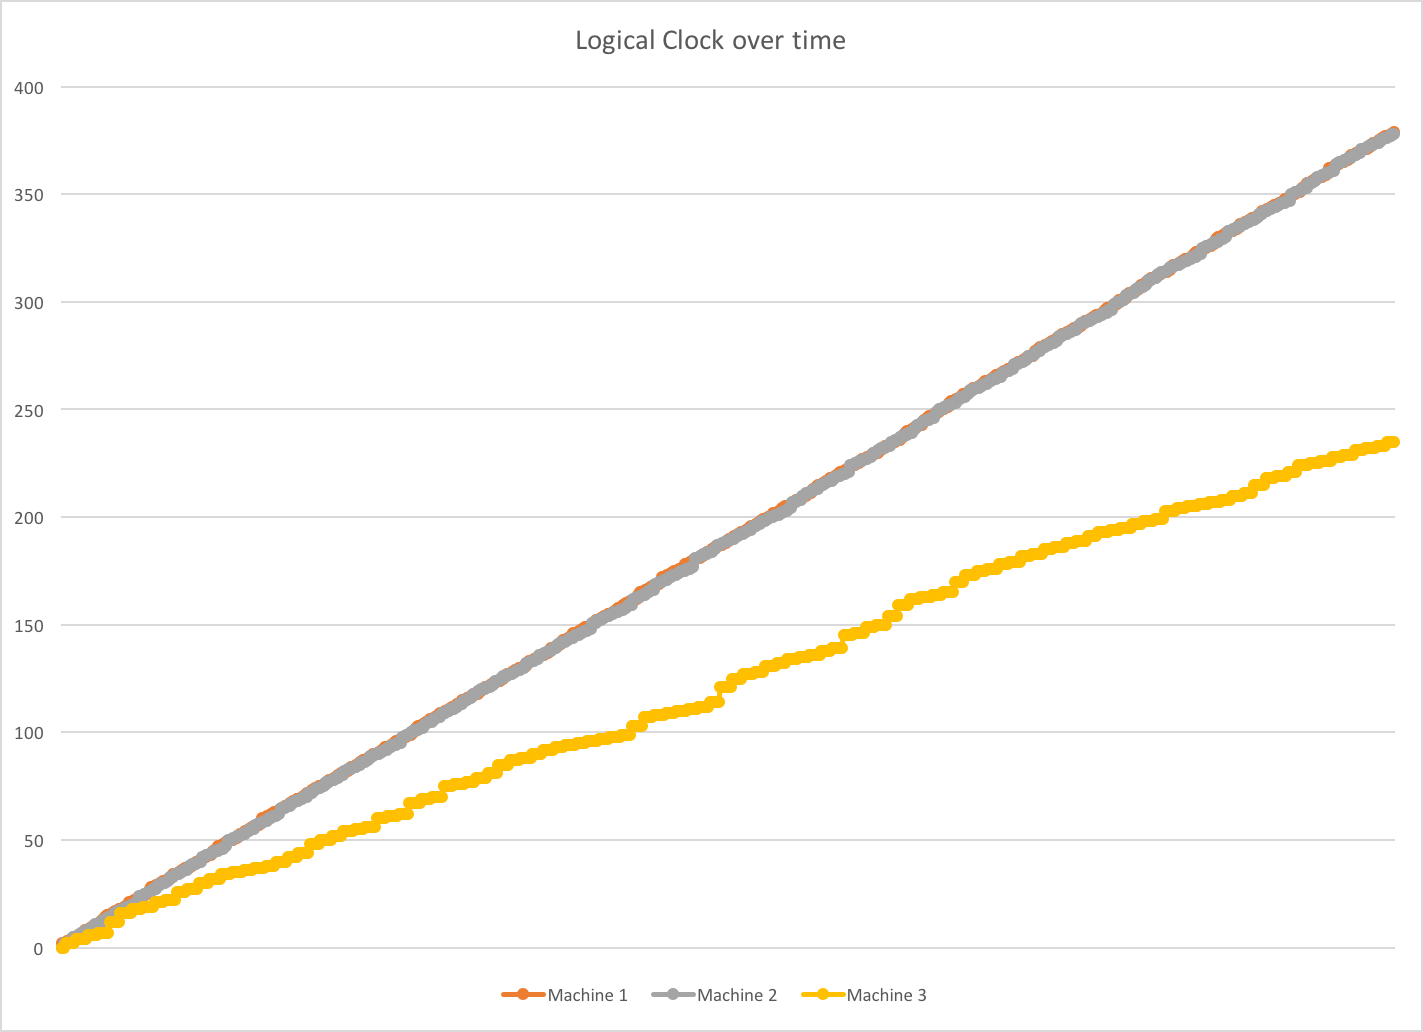
\includegraphics[width=0.5\textwidth]{{{pictures/1457671089.64_lc}}}
    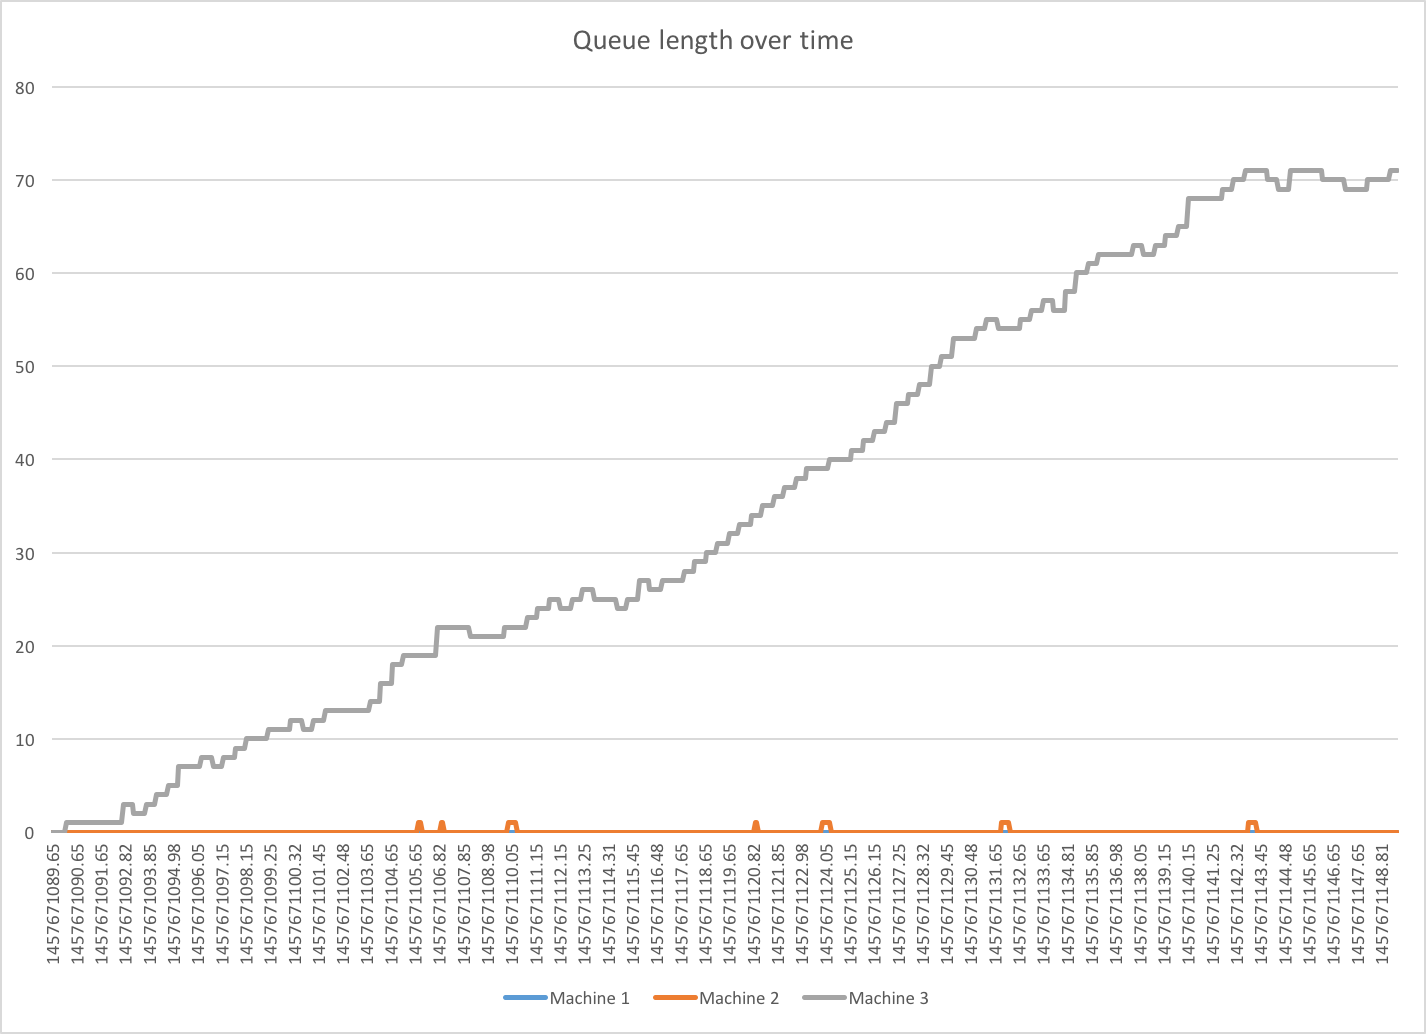
\includegraphics[width=0.5\textwidth]{{{pictures/1457671089.64_queue}}}
\end{figure}


For the second one, we are making internal events more likely. That means that the processes will increase their logical clock values without synchronizing with one another as much. However, since there is less communication, when there is the occasional communication, they will sync up. So, we would expect to see larger jumps, but the process's logical clocks largely keeping up with one another. This is exactly what happens, and we can see this in \ref{fig:ex3}. The case with internal=35 has the same general behavior, except the jumps are larger, as is expected.


\begin{figure}[!ht]
  \label{fig:ex3}
  \centering
    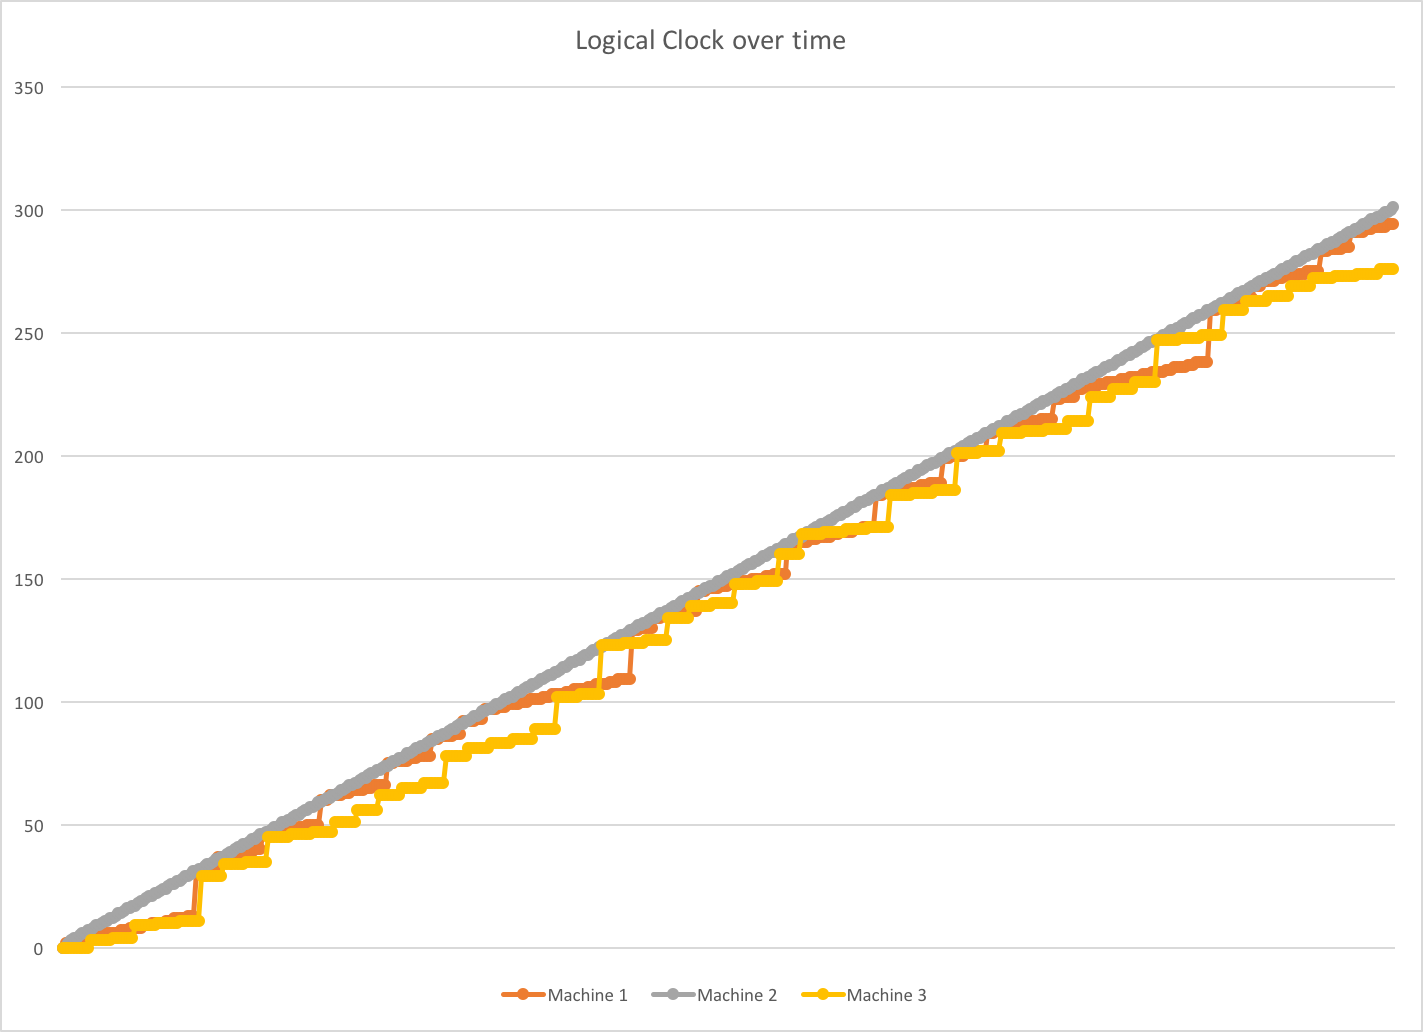
\includegraphics[width=0.5\textwidth]{{{pictures/1457671149.97_lc}}}
    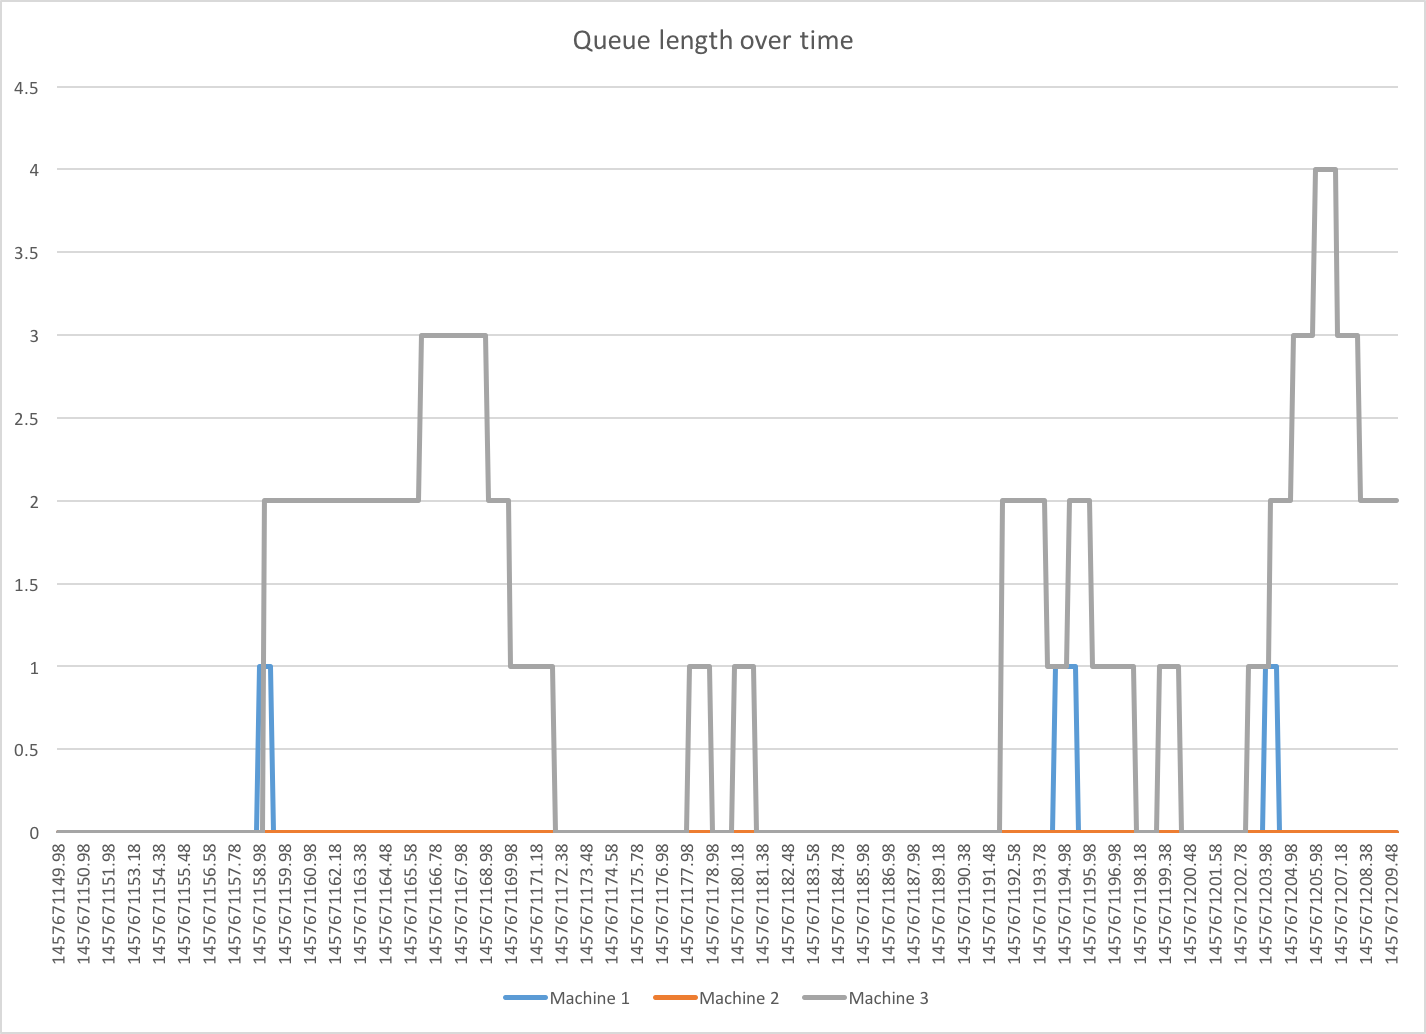
\includegraphics[width=0.5\textwidth]{{{pictures/1457671149.97_queue}}}
\end{figure}

\subsection{Experiments 3}
In this set of experiments, we maintain internal, but change the max clock speed for a process. This allows us to see what happens with differences between process speed is much higher (say, an order of magnitude), or much lower, where the number of ticks per second is just 1, 2, or 3. So, in this set of experiments, we set the probability of an internal event to the default .7, but we varied the maximum clock speed to be 3, 10, and 20, rather than the default of 6.

For the max speed of 3, we expected that the three processes would essentially all have the same speed, and would thus be able to keep up with one another in terms of logical clock speed. Though this is generally what happened, there was actually some lag in the logical clock values for one the processes. We believe this is because that process got a clock speed of 1 per second, which was half of the other two. So, it seems that the ratio of process speeds is the critical element in determining whether a process can consistently keep up, which makes sense in retrospect. You can see this in \ref{fig:ex4}.


\begin{figure}[!ht]
  \label{fig:ex4}
  \centering
    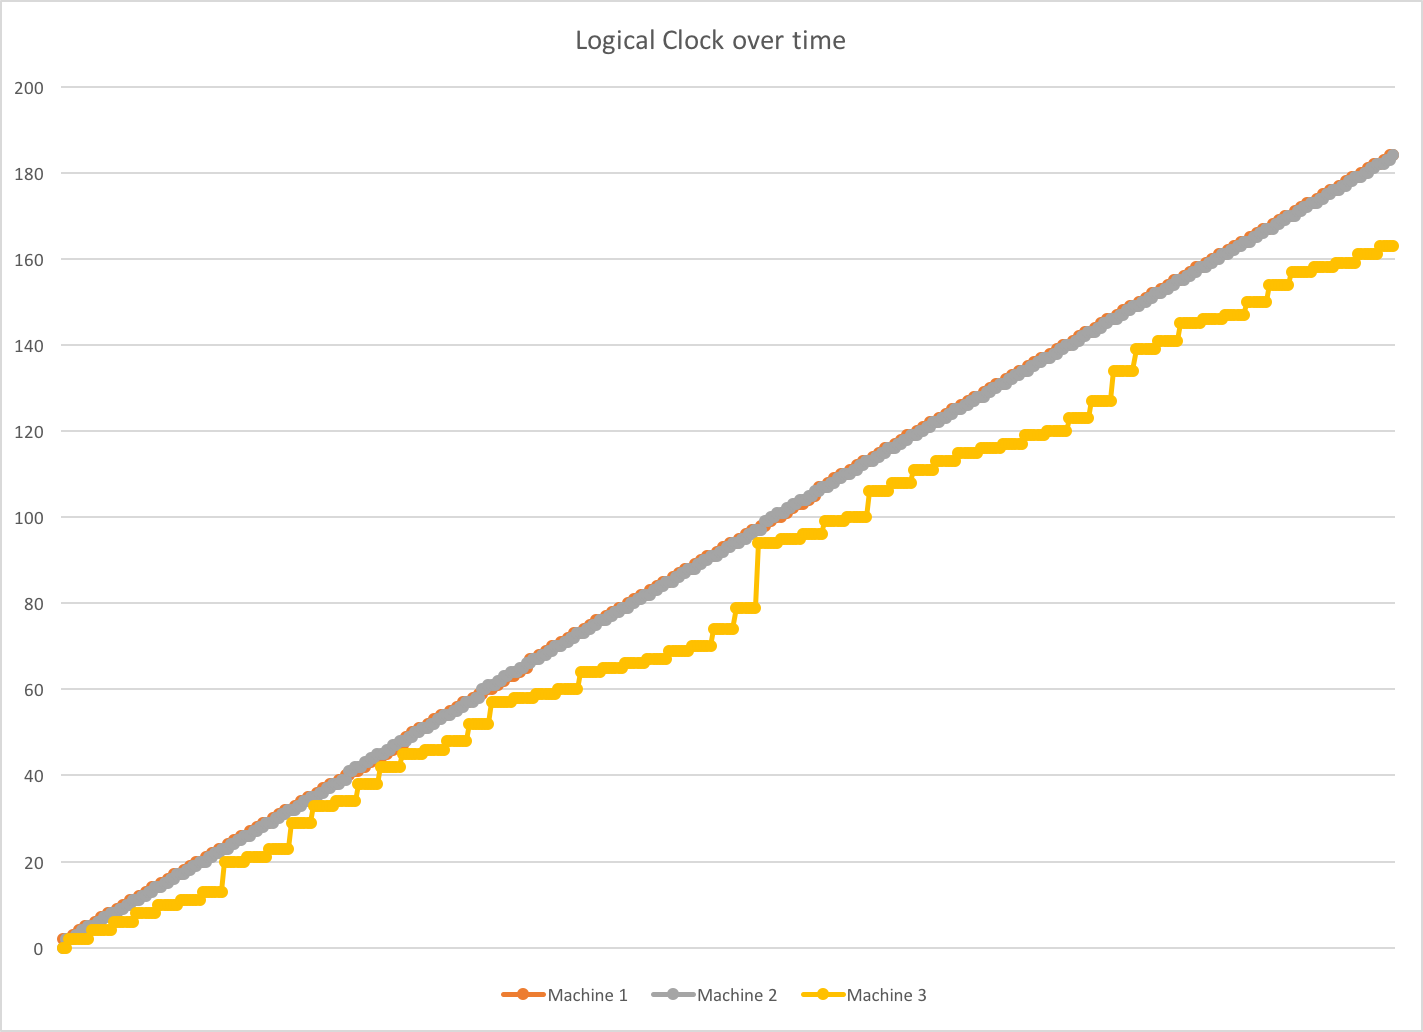
\includegraphics[width=0.5\textwidth]{{{pictures/1457671270.55_lc}}}
    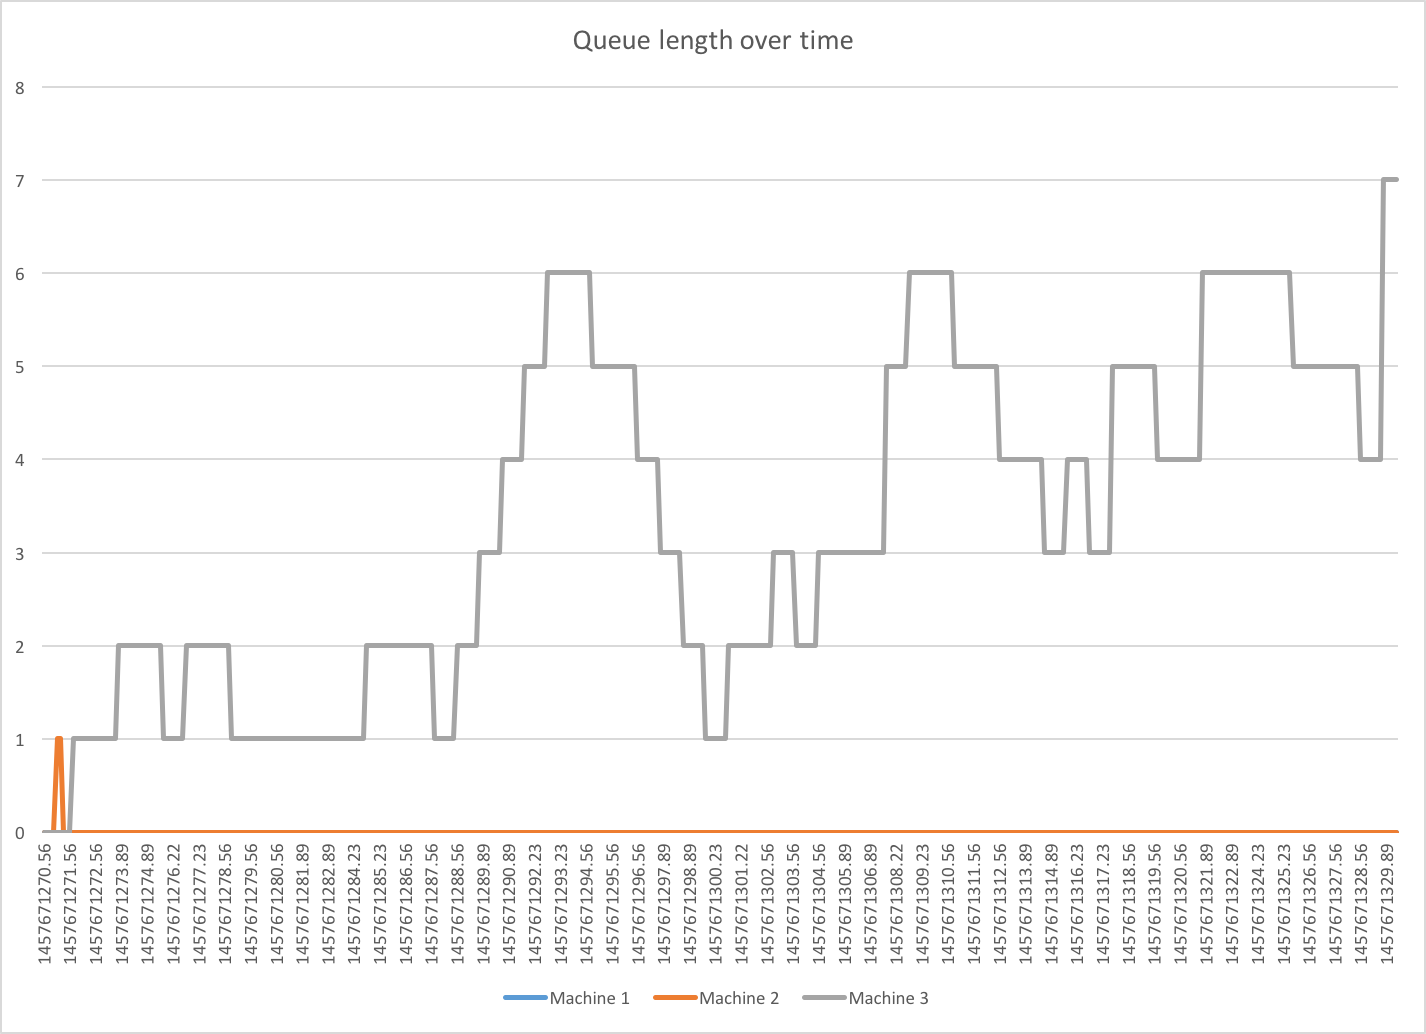
\includegraphics[width=0.5\textwidth]{{{pictures/1457671270.55_queue}}}
\end{figure}


For the max speed of 10, our sampled values tended to be close to one another, so all of the processes ran at the very similar speed. Thus, the processes logical clocks were able to keep up with one another and the queues were small. You can see this in \ref{fig:ex5}.

\begin{figure}[!ht]
  \label{fig:ex5}
  \centering
    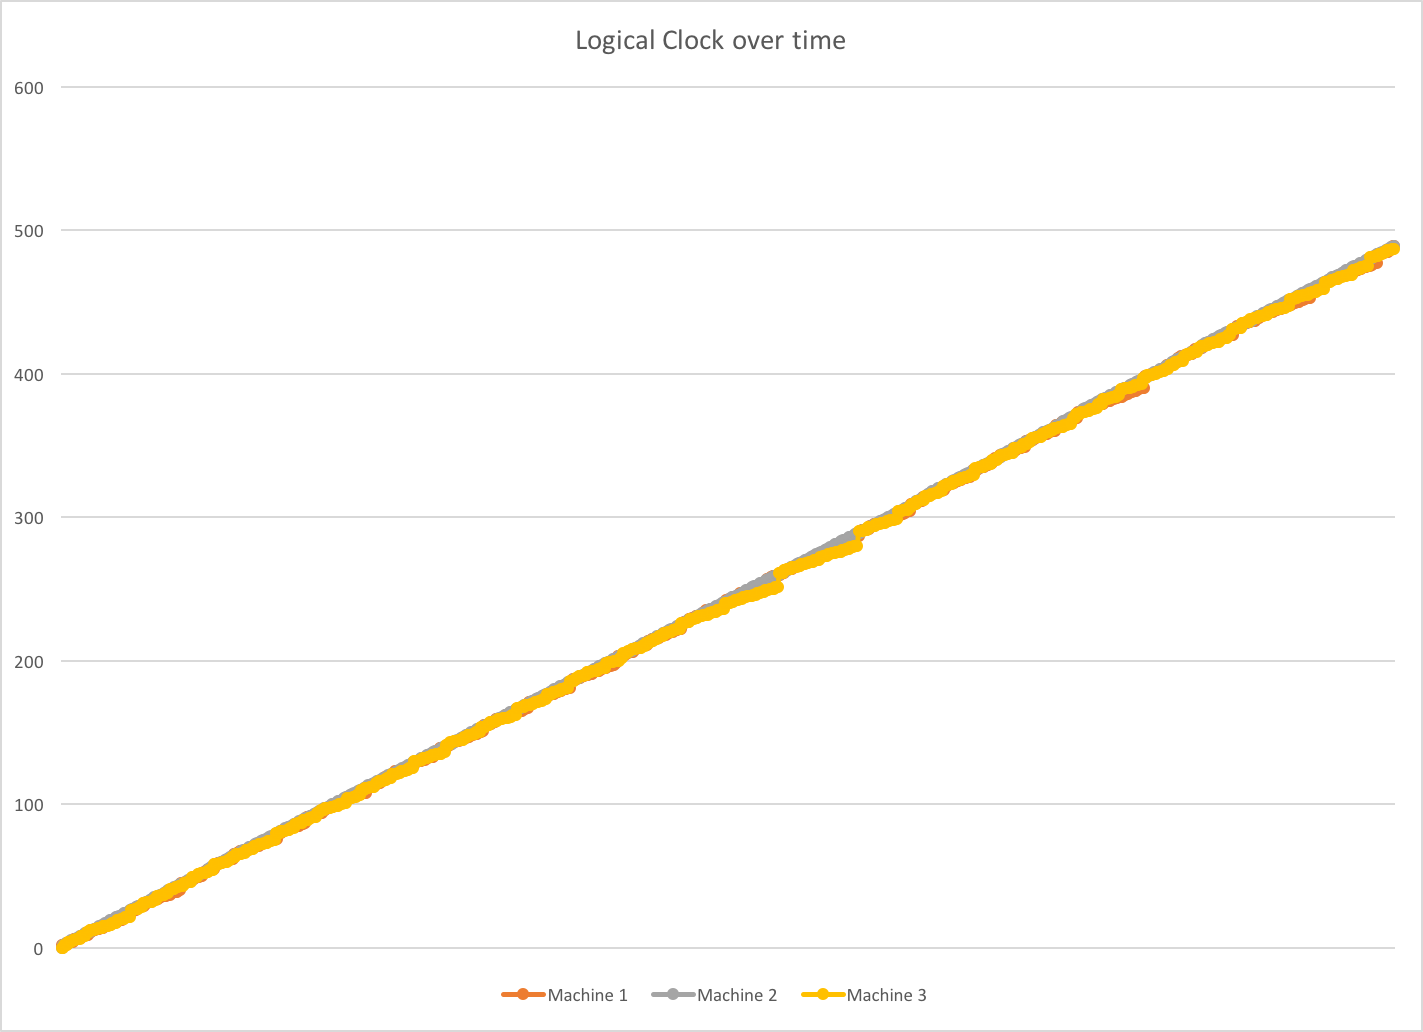
\includegraphics[width=0.5\textwidth]{{{pictures/1457671330.86_lc}}}
    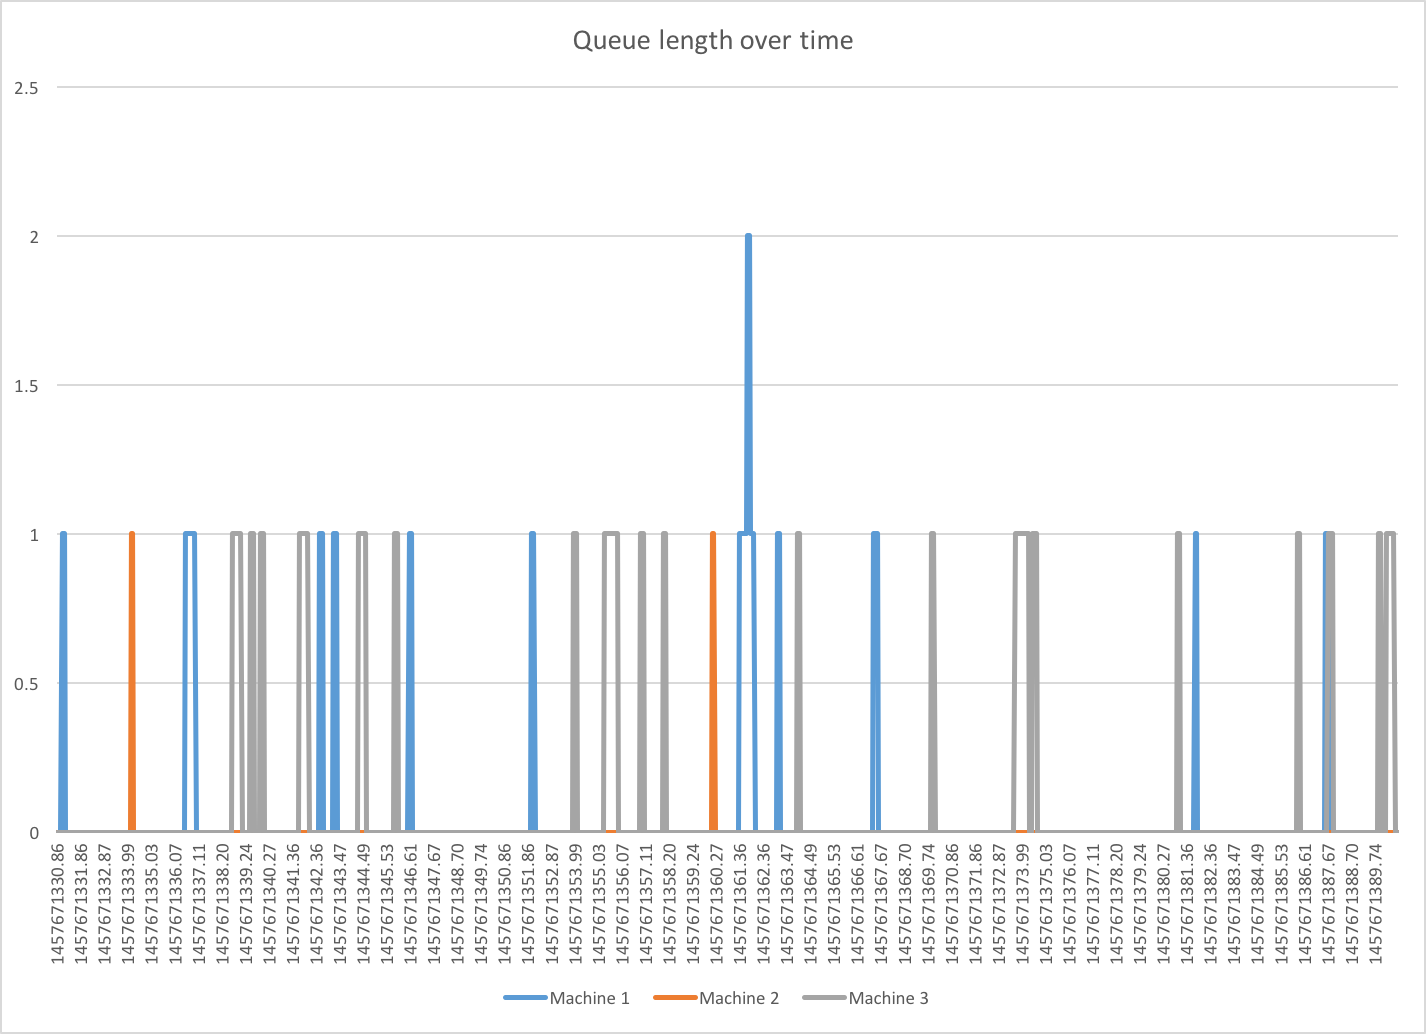
\includegraphics[width=0.5\textwidth]{{{pictures/1457671330.86_queue}}}
\end{figure}

However, with the max speed of 20, our sampled clock speeds were much more varied. In particular, one of the processes had a clock speed of 10 ticks per second, and the other was 1 tick per second, giving an order of magnitude difference. In this case, we can see that slow process is simply not able to keep up, since it cannot process everything that comes into its queue. You can see the results for this in \ref{fig:ex6}.

\begin{figure}[!ht]
  \label{fig:ex6}
  \centering
    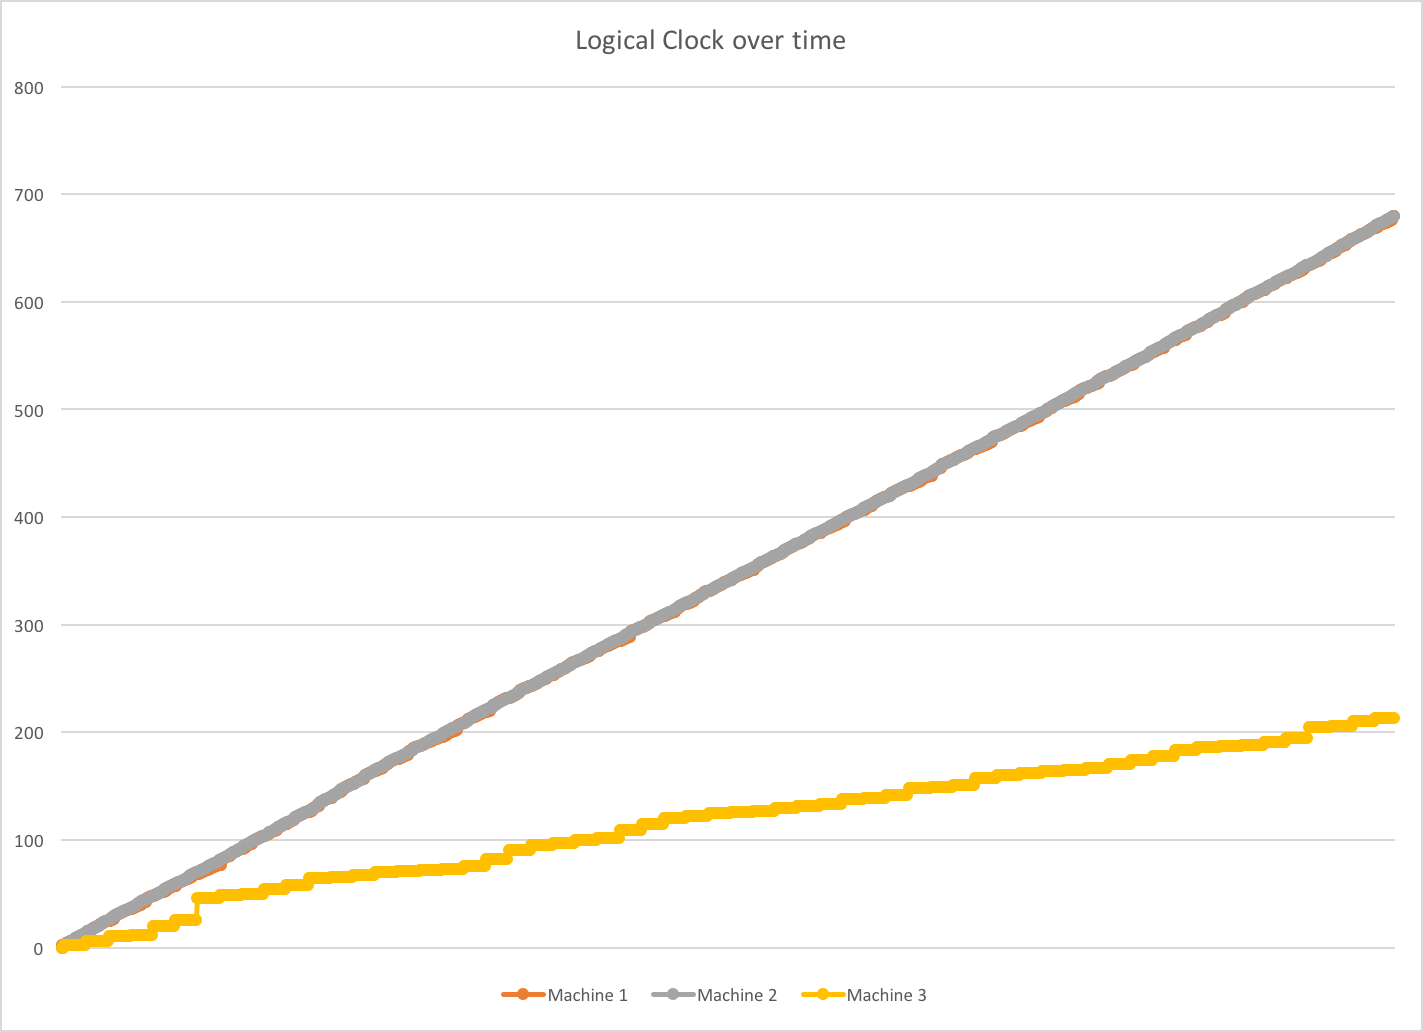
\includegraphics[width=0.5\textwidth]{{{pictures/1457671391.12_lc}}}
    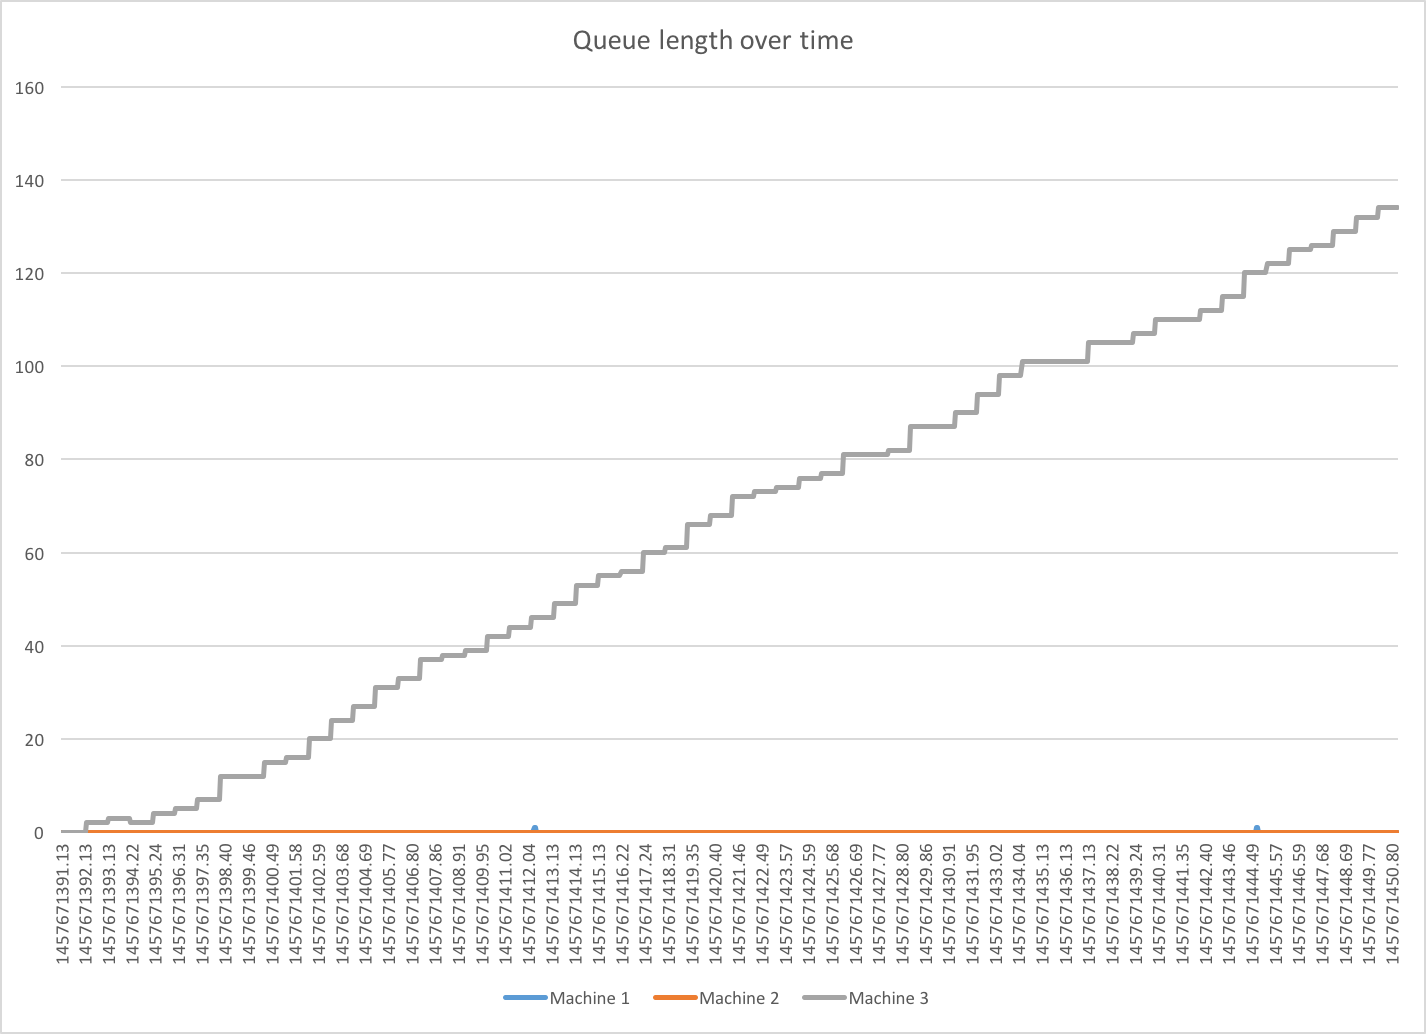
\includegraphics[width=0.5\textwidth]{{{pictures/1457671391.12_queue}}}
\end{figure}

\subsection{Experiments 4}

In the last set of experiments, we looked at what happens when we change both the max speed and the internal event probability. In particular, we wanted to see how these two changes could interact with one another, and perhaps lead to one cancelling the other out, or augmenting the other.

Here are the configurations we tried:

\begin{center}
\begin{tabular}{ | c | c | }
\hline
max speed = 3 &P(internal) = 2/5 \\
max speed = 3 &P(internal) = 12/15 \\
max speed = 10 &P(internal) = 2/5 \\
max speed = 10 &P(internal) = 12/15 \\
max speed = 20 &P(internal) = 2/5 \\
max speed = 20 &P(internal) = 12/15 \\
\hline
\end{tabular}
\end{center}

Rather than talking about each of these separately, we will discuss the high-level takeaways from these configurations. For some of these, we observed and amplified effect from before, and some of the processes were simply inundated and could not keep up with the others. For example, consider the max speed = 20, P(internal) = 5 case (\ref{fig:ex7}). In this one, the slowest process had to both deal with the fact that there was tons of communication because of the low chance of an internal event in any process, and there was a very high max possible clock speed. So, you can see that the logical clock value for one process lags way behind the others, and the queue is very long (300+). On the other hand, we can see that having a max speed = 20 and internal = 15 can mitigate the effects of a very large max speed. In this case, we still had one process that was an order of magnitude faster than another. However, the high probability of internal events means that there was less communication, smaller queues, and it was easier for the processes to stay caught up with one another. You can see this in \ref{fig:ex8}.

\begin{figure}[!ht]
  \label{fig:ex7}
  \centering
    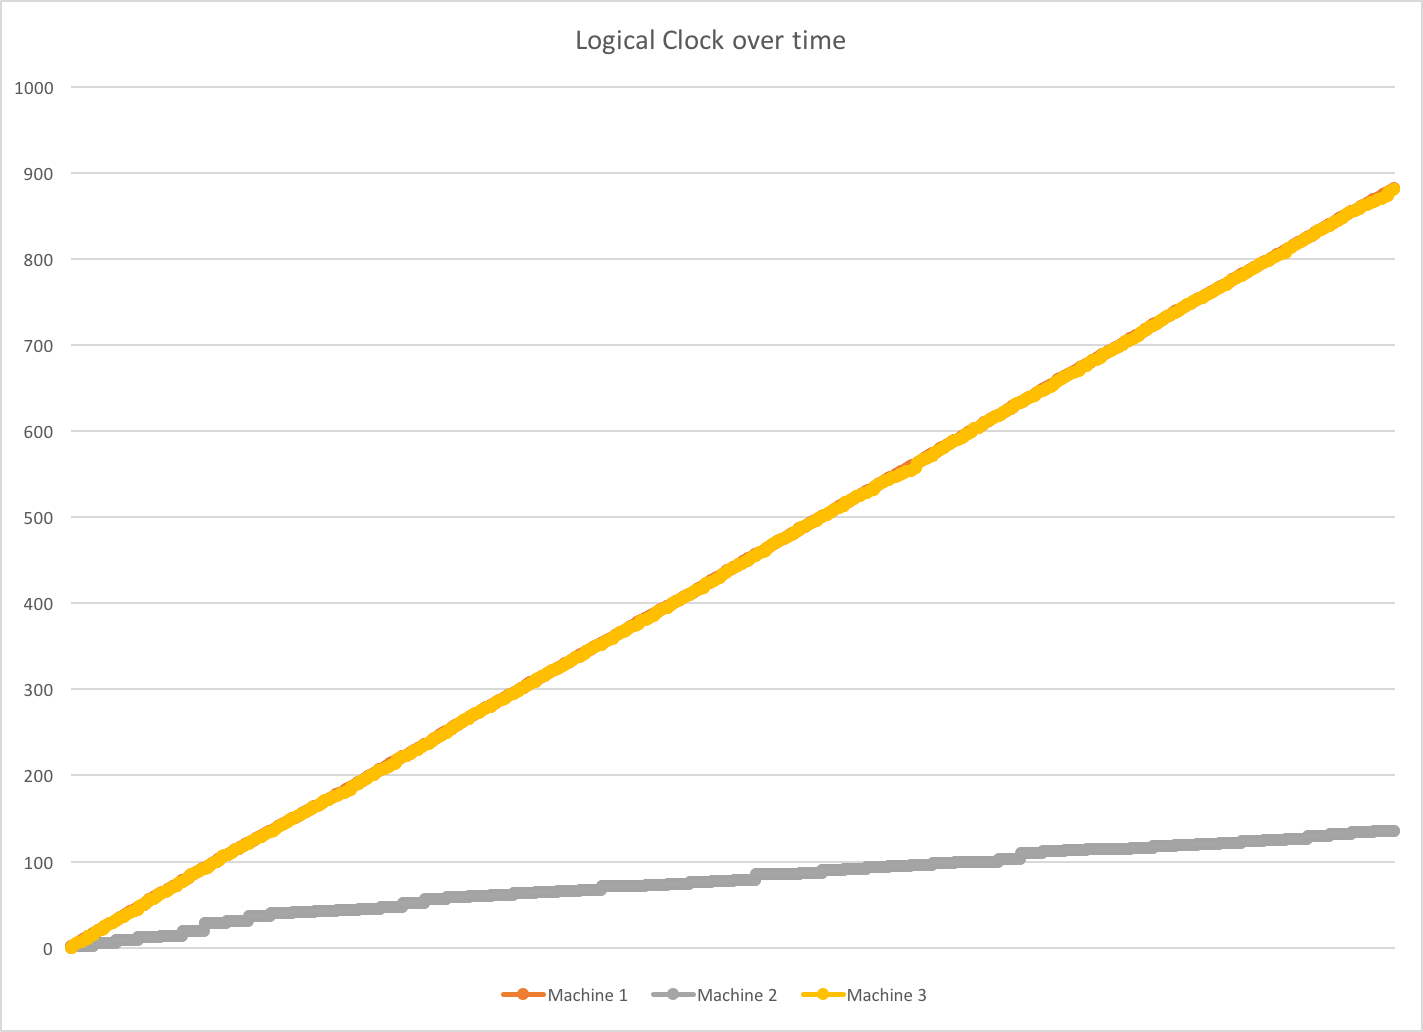
\includegraphics[width=0.5\textwidth]{{{pictures/1457671692.8_lc}}}
    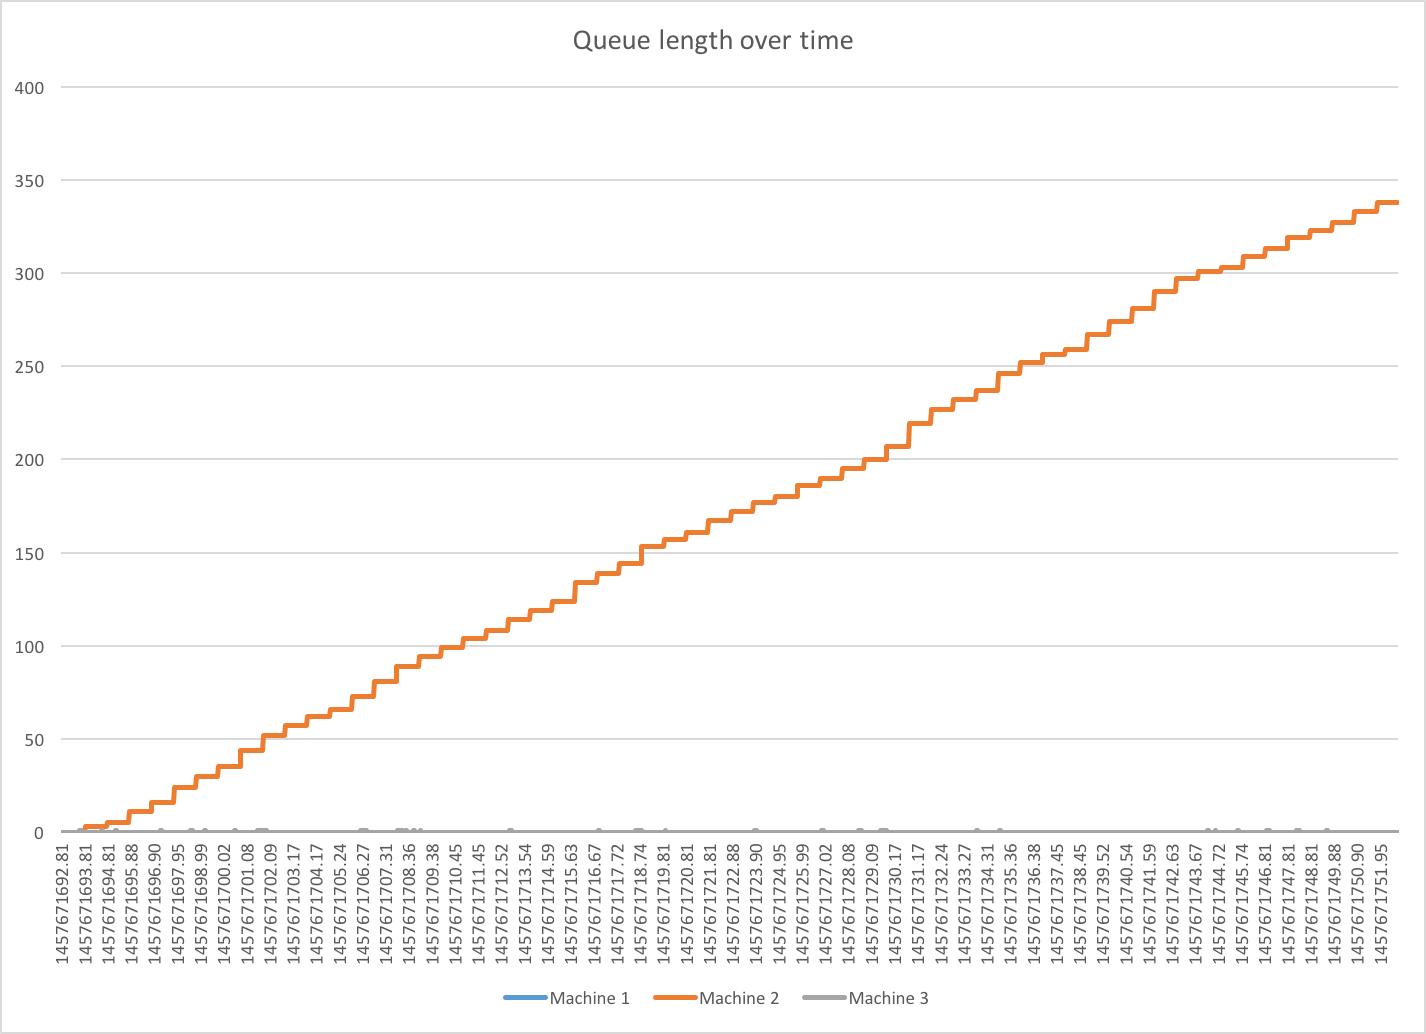
\includegraphics[width=0.5\textwidth]{{{pictures/1457671692.8_queue}}}
\end{figure}

\begin{figure}[!ht]
  \label{fig:ex8}
  \centering
    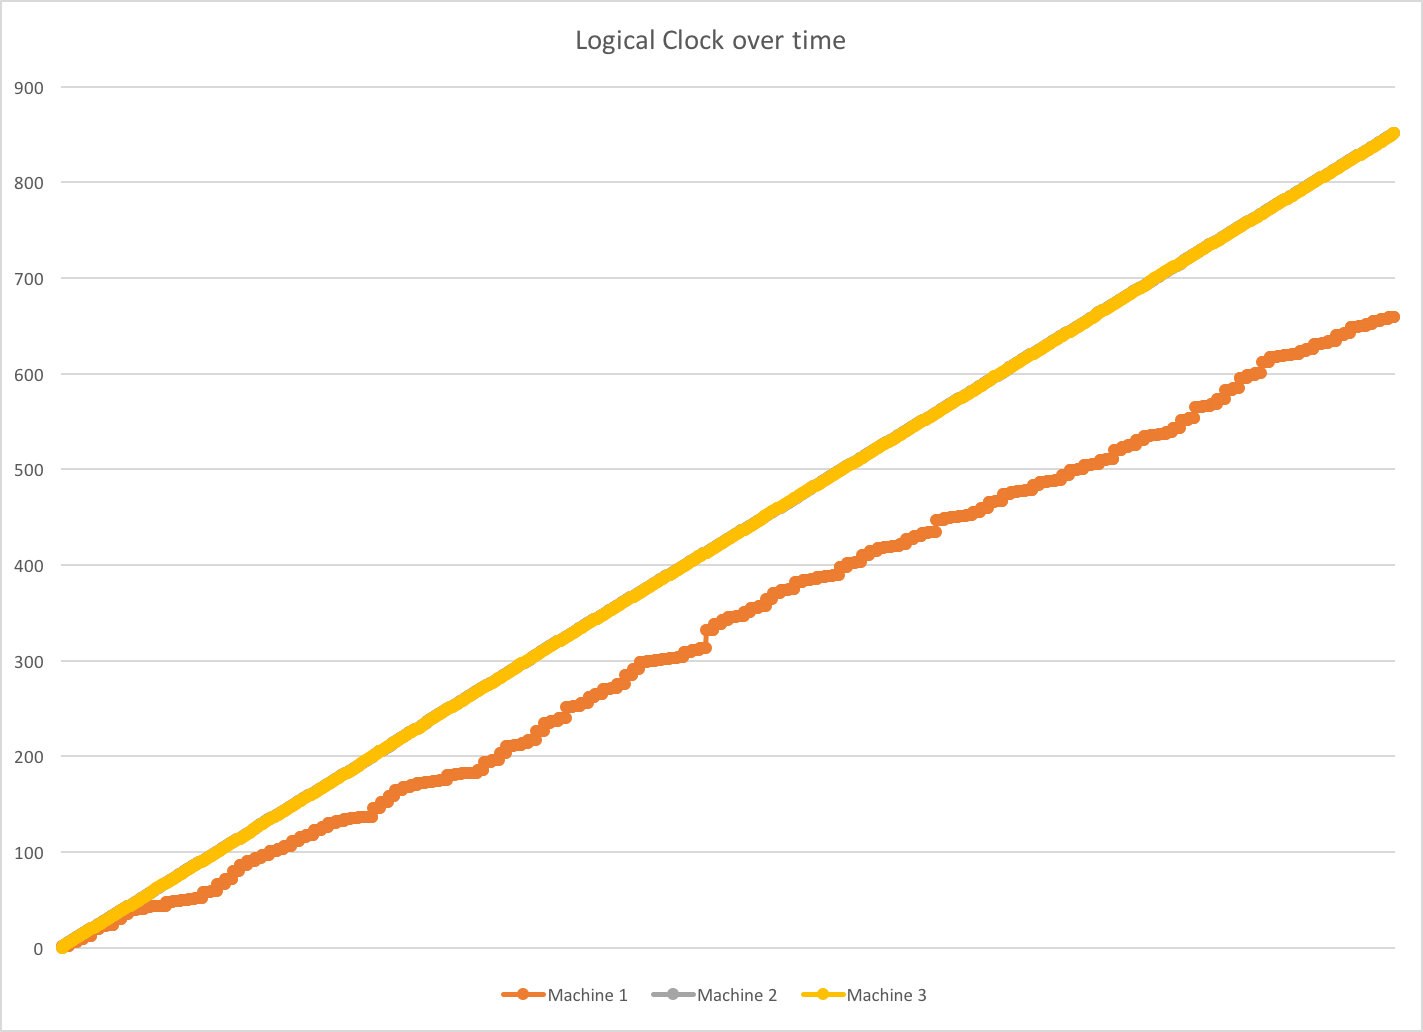
\includegraphics[width=0.5\textwidth]{{{pictures/1457671753.09.lc}}}
    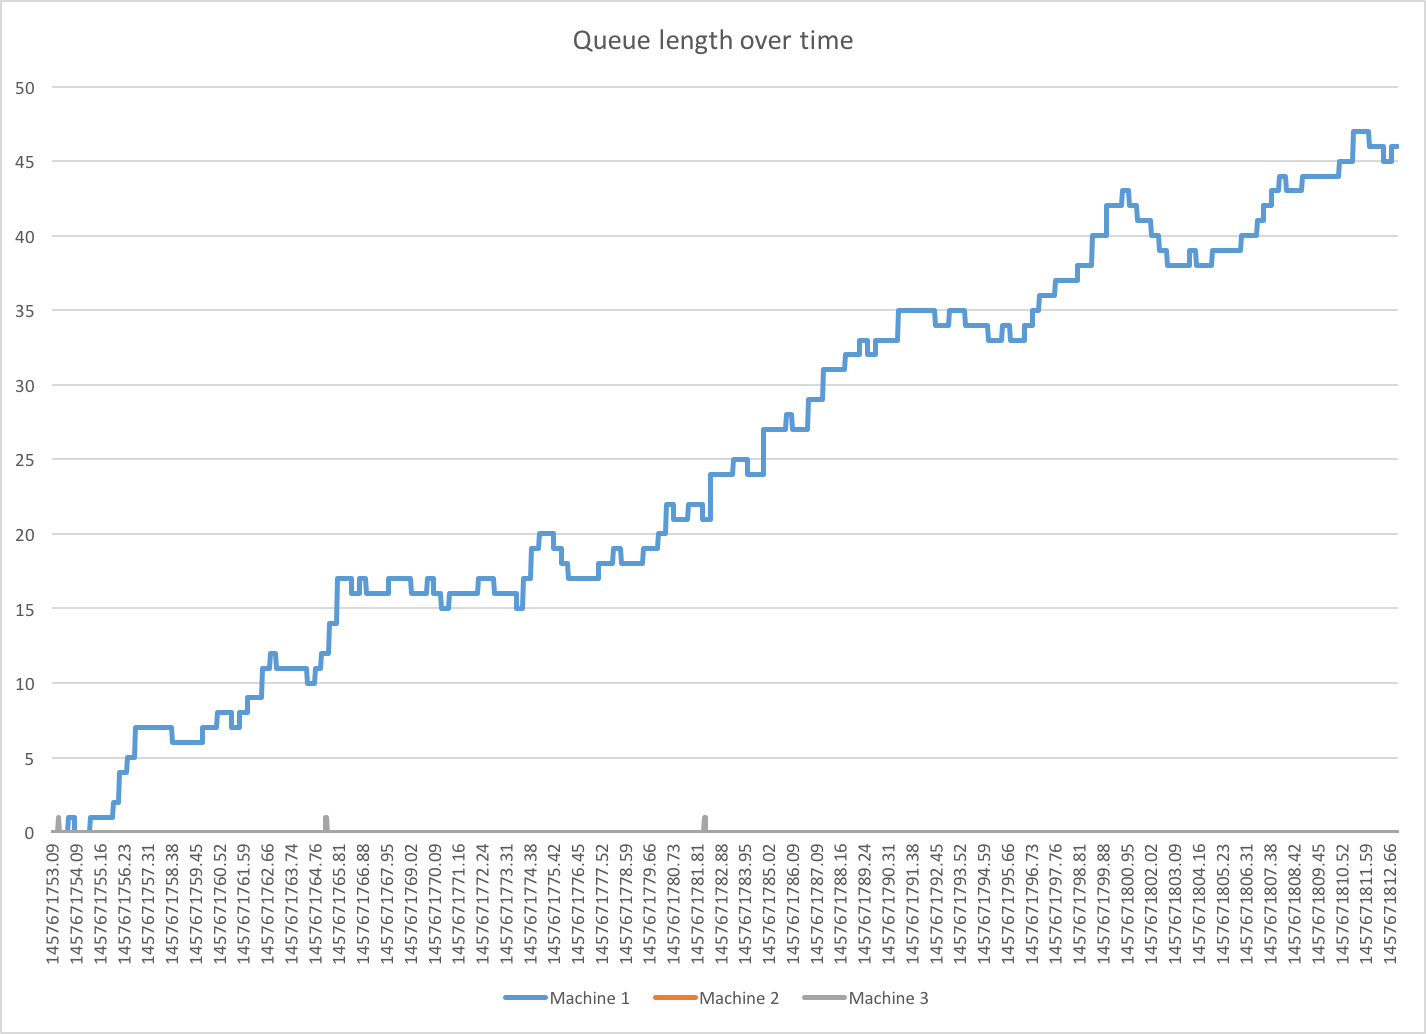
\includegraphics[width=0.5\textwidth]{{{pictures/1457671753.09.queue}}}
\end{figure}

\section{Conclusion}
Overall, we generally found that under many conditions, one of the processes will significantly lag behind the others in terms of logical clock value. In particular, we can create this occurrence by having very high max speed values, which would likely lead to one process being much faster than the other, and thus the other being left behind.  We can also do this by decreasing the amount of internal events, and thus increasing the amount of interprocess communication, which would also lead to large queues of messages in the slowest process.


% that's all folks
\end{document}


